\chapter{Fundamentação Teórica}
\label{cap:funcamentacao:teorica}
\section{Energia fotovoltaica}
O efeito fotovoltaico, observado por Edmond Bequerel em 1939, consiste no aparecimento de uma diferença de potencial nos extremos de um semicondutor, quando esse absorve  a luz.\cite{} São várias as vantagens da energia solar fotovoltaica:
\begin{itemize}
\item a matéria prima é inesgotável
\item não há emissão de poluentes durante a geração da eletricidade
\item os sistemas podem ser instalados em todo o globo
\end{itemize}


Um sistema fotovoltaico é uma fonte de potência elétrica, na qual as células fotovoltaicas transformam radiação solar diretamente em energia elétrica. Sistemas fotovoltaicos são utilizados em locais inóspitos como: espaço, desertos, selvas, regiões remotas, entre outros. Este tipo de sistema pode ser classificado em relação a sua geração e entrega de energia elétrica:
\begin{itemize}
\item Sistemas isolados
\item Sistemas conectados à rede(\textit{On-grid})
\end{itemize}

Dentre essas duas classificações, ainda existem subdivisões quanto ao seu uso e construção, como pode ser observado no diagrama abaixo: 
\begin{figure}[H]
    \centering
    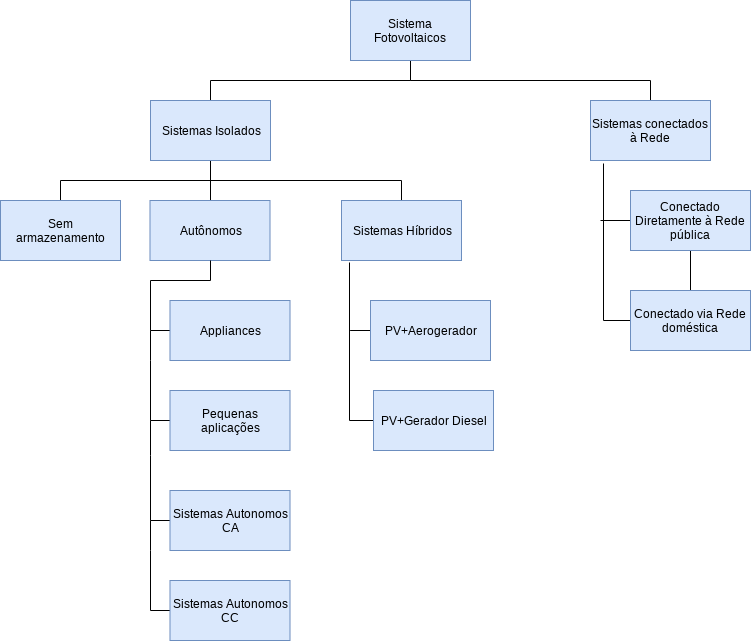
\includegraphics[width=1.0\textwidth]{figuras/sistemasFoto.png}
    \caption{Tipos de sistemas fotovoltaicos}
    \label{fig:caminho-objetos-scheduling}
\end{figure}

Um sistema fotovoltaico isolado não possui conexão com a rede de distribuição, podendo ser híbridos: quando existe a adição de outra fonte de energia, tais como geradores a combustível fóssil ou turbinas eólicas, ou autônomos, sendo esses constituídos apenas dos painéis solares. Já um sistema conectado à rede(\textit{On-Grid}) todo potencial gerado é escoado para a rede, sendo esses, mais eficientes que os sistemas autônomos, mesmo não tendo sistemas de armazenamento de energia, além de serem mais baratos.

Para utilizar um sistema fotovoltaico autônomo é necessário realizar um estudo sobre os equipamentos a serem utilizadas, suas demandas energéticas, quantidades, além de um estudo sobre quais os componentes que mais se adaptariam a tal projeto. Inicialmente deve-se calcular o gasto total diário baseando-se em quantos Watts/hora cada equipamento gasta e por quanto tempo ele será utilizado durante o dia. Para tal, podemos utilizar a seguinte fórmula:
% https://www.codecogs.com/latex/eqneditor.php?lang=pt-br
\[Consumo = \sum_{1}^{n}\left ( qtd.W \right )h\]

Onde temos que o consumo é proveniente da quantidade(\textit{qtd}) de equipamentos vezes a potência em \textit{Watts}(\textit{W})por hora vezes as horas(\textit{h}) de utilização. Em seguida, deve-se calcular a \textit{Potência instantânea} que o inversor de corrente deverá transferir as baterias, para isso, calcula-se a soma da potência dos equipamentos ligados simultaneamente.
\[Potência instantânea = \sum_{1}^{n} qtd.W  \]

Onde temos que o  potência instantânea é proveniente da quantidade(\textit{qtd}) de equipamentos vezes a potência em \textit{Watts}(\textit{W})por hora. Deve-se calcular uma folga para o inversor, tendo-se em mente que trabalham na faixa de 50\% e 70\% de sua capacidade, logo:
\[F_{max}=\frac{P.I}{0.5}\] e \[F_{min}=\frac{P.I}{0.7}\]

Dado os resultados, pode-se escolher um inversor autônomo que opere dentre essa faixa, tendo em vista a especificação de qual sua eficiência máxima, pois deve-se calcular o valor da energia gerada pelo sistema diariamente tendo-se em vista o autoconsumo do inversor:
\[ED =\frac{Consumo}{Eficiência Máxima}\]

A partir desses dados, é possível calcular a energia real da instalação:
\[ER=\frac{ED}{R}\]
Onde R é o Rendimento Global, calculado mediante fatores de perdas possíveis, normalmente assumindo o valor de 89\%(0,89). Por fim, calcula-se o valor da capacidade útil do banco de baterias, assumindo que \textbf{N} seja o valor de dias de autonomia do sistema e \textbf{Vi} sendo o valor da tensão
\[CU=\frac{ER*N}{Vi}\]
Vale a pena ressaltar que as baterias do sistema não podem ser descarregadas em sua totalidade, a carga real do sistema é dada por: 
\[CR=\frac{CU}{PD}\]
PD sendo o valor da profundidade da descarga da bateria. Por fim calcula-se o número de baterias a serem usadas, tanto em pararelo quanto em série:
\[NB=\left ( \frac{CR}{CN} \right )*\left ( \frac{Vi}{VB} \right )\]
Vb é a tensão nominal e CN a capacidade da bateria.

Em posse as características do sistema fotovoltaico idealizado e com os cálculos acima descritos, fica factível a construção de um sistema para suprir suas necessidades e respeitando as características dos seus componentes.

\section{Computação Autônoma}

Como sistemas tem se tornado cada vez mais interconectados e diversos, arquitetos estão cada vez menos capazes de antecipar e construir as interações entre os componentes, deixando esses problemas para serem resolvidos em tempo real. Logo, os sistemas ficaram gigantescos e muito complexos até mesmo para o mais qualificado dos integradores de sistema para instalar, configurar, otimizar, manutenir e conectar. A única opção restante é computação autônoma: sistemas que conseguem gerenciar a si mesmos dados certos objetivos.\cite{Kephart2003}

Um dos pilares essenciais de um sistema autônomo é a capacidade sensorial do mesmo, onde o habilita a observar o contexto externo. É também de suma importância que o sistema tenha propósito e \textit{Know-how} para continuar operando sem ajuda externa, operação essa que é ditada pela lógica embutida responsável pelas tomadas de decisão para que o proposito e seus objetivos sejam alcançados, baseando-se também, no poder de interpretação dos dados provenientes dos sensores. Como é observado na figura \ref{fig:modelo-conceitual}, o sistema deve ser capaz de produzir saídas, dado as entradas(objetivos, dados) e as informações provenientes dos sensores, tomando as corretas decisões e adaptando-se as mudanças de contexto.

\begin{figure}[H]
    \centering
    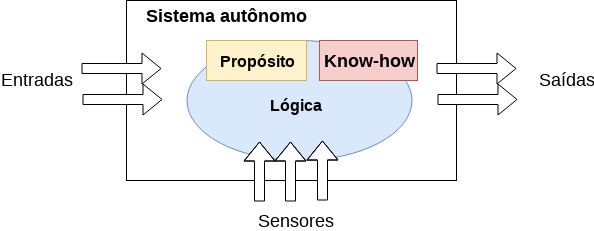
\includegraphics[width=0.7\textwidth]{figuras/autonomo.png}
    \caption{Modelo conceitual}
    \label{fig:modelo-conceitual}
\end{figure}


A essência de um sistema autônomo é o auto-gerenciamento, sendo este capaz de ajustar sua operação para comportar as mudanças de cargas de trabalho, demandas e condições externas, além de possíveis falhas de hardware ou software. O sistema deve ser capaz de compilar informações sobre uso de hardware, desempenho dos softwares e componentes a fim de ajudar em decisões futuras, sendo esses também, capazes de automaticamente reverter essas decisões se julgar que o resultado não mantenha ou melhore os padrões de disponibilidade do mesmo.

Sistemas autônomos são capazes de configurar-se automaticamente de acordo com as prioridades de alto nível que especificam o que é desejado do sistema. Ao incorporar novos componentes ao sistema, o mesmo deve se adaptar a adição, reconfigurando os demais componentes para que todos continuem a funcionar em sinergia. Além disso, esses sistemas devem, de forma continua, procurar modos de otimizar sua operação, buscando a melhor combinação de parâmetros e buscando a continua atualização dos componentes, isso, devido a grandiosa complexidade desses sistemas demandarem horas de trabalho de um especialista para que sejam otimizados.

A tarefa de encontrar um \textit{bug}, descobrir suas causas e, por fim, construir uma solução pode consumir inúmeras horas de trabalho de uma equipe de programadores. Um sistema autônomo deve detectar, diagnosticar e resolver certos problemas que encontrar ou, se necessário, notificar os administradores do problema. O sistema é capaz de realizar tal tarefa, dado o conhecimento do próprio funcionamento e da performance que pode alcançar. Além disso, o sistema pode se proteger de ataques que possam acarretar perdas de performance e de disponibilidade, bem como utilizar seus sensores para verificar passiveis problemas e tomar decisões de como evita-los.

\section{Arduino}
Arduino é uma plataforma eletrônica de código aberto,  concebida para ser fácil de usar, tanto em termos de hardware, como de software. Por essa natureza, Arduino é indicado para hobbistas, estudantes e professores, pois além de simples, é de baixo custo, multiplataforma e possui uma gama enorme de software e hardware open-sorce.\cite{Mohammed2017}

\begin{figure}[H]
    \centering
    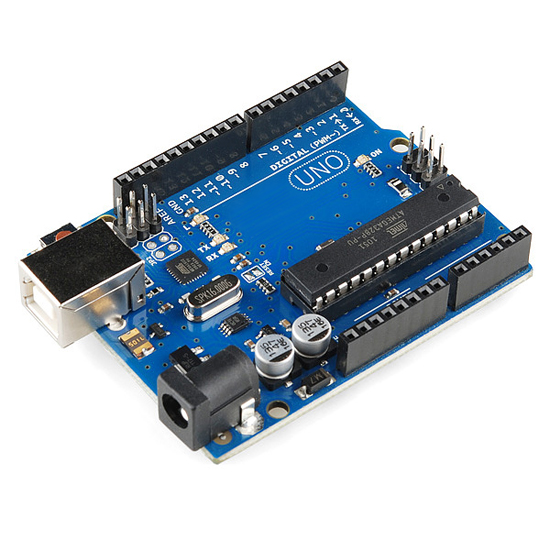
\includegraphics[width=0.7\textwidth]{figuras/Arduino_Uno_R3.png}
    \caption{Uma das várias versões do Arduino: a Uno R3}
    \label{fig:arduino-uno}
\end{figure}

A família Arduino é baseada no micro controlador ATmega32 de 8-bits, com clock de 16mhz, várias entradas digitais e analógicas para IO, comunicação serial, USB e ICSP. Para sua operação, Arduino requer uma voltagem de 7 a 12V. Possui 35kb de memória, sendo essas: 32kb de memória flash, onde os programas são carregados, 2kb de SRAM(static random access memory) para manipulação de variáveis e \textit{erasable read only memory}(EEP-ROM) de 1kb  onde ficam os dados que devem ser persistidos. No site oficial do Arduino\footnote{https://www.arduino.cc/} encontra-se disponível também a IDE(Integrated Development Environment) oficial, onde é possível editar e compilar códigos, bem como comunicar-se com a placa.

Um Arduino pode ser conectado a vários tipos de \textit{shields} para inúmeras aplicações, desde o controle de motores, módulos GPS, Wifi e Bluetooth. Por toda essa capacidade, Arduino vem crescendo dentro das indústrias também, onde um estudo feito por UBM\footnote{http://bd.eduweb.hhs.nl/es/2014-embedded-market-study-then-now-whats-next.pdf} em 2014, mostrou que 19\% dos profissionais questionados consideravam a utilização do Arduino nos próximos projetos.
\section{Raspberry PI}

Segundo o site do fabricante\footnote{https://www.raspberrypi.org/help/what-\%20is-a-raspberry-pi/} , Raspberry Pi é um computador de baixo custo, pequeno tamanho que pode ser conectado diretamente a um monitor ou aparelho de televisão. É capaz de rodar um sistema operacional, comumente o Raspbian, uma versão famoso sistema operacional Debian, criada especificamente para o Raspberry Pi. Apesar do pequeno tamanho, é possível executar tarefas de um computador normal, tais como programar, navegar na internet, assistir filmes em alta resolução, etc. 

A placa apresenta, na sua versão 2, um processador quad-core de 900mhz  Broadcom BCM2836 quad core Cortex A7, 1 GB de memória RAM, portas USB, Ethernet, cartão MicroSD, saía de áudio e HDM. Dadas essas características, essa versão é mais indicada a projetos que necessitem de mais processamento, muitas vezes usada como "cérebro" em projetos de Internet das Coisas.

\begin{figure}[H]
    \centering
    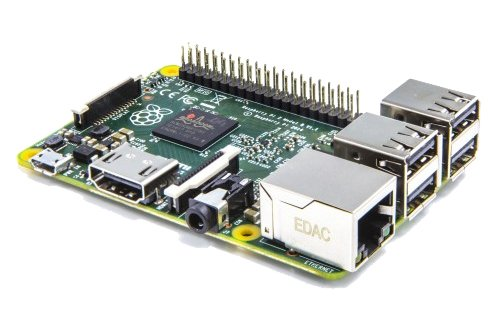
\includegraphics[width=0.7\textwidth]{figuras/raspberrypi2.jpg}
    \caption{Raspberry Pi 2}
    \label{fig:raspberry-pi}
\end{figure}

\section{Mapas georreferenciados}
Para \cite{Meng2014}, georreferenciamento é "alinhar dados geográficos com um sistema de coordenadas conhecidos para que possa ser pesquisado, visualizado e analisado com outros dados geográficos". O processo de identificar um objeto geográfico e relaciona-lo a uma locação geográfica é chamado de \textit{matching}\footnote{casar,igualar, combinar}. Georreferenciamento  normalmente usa um sistema de referencia chamado \textit{WGS-84}, que constrói coordenadas padronizadas para a terra, em adição, alguns dispositivos de navegação são utilizados para coletar dados e atrela-los ao processo de construção do mapa. A combinação de dados provenientes de GPS em combinação com \textit{WGS-84}, podem referenciar a um certo ponto geográfico no mapa \ref{fig:mapa:georef}. Esse tipo de mapa pode combinar dados e imagens capturados por satélite, aeronaves ou veículos aéreos não tripulados. 

\begin{figure}[H]
    \centering
    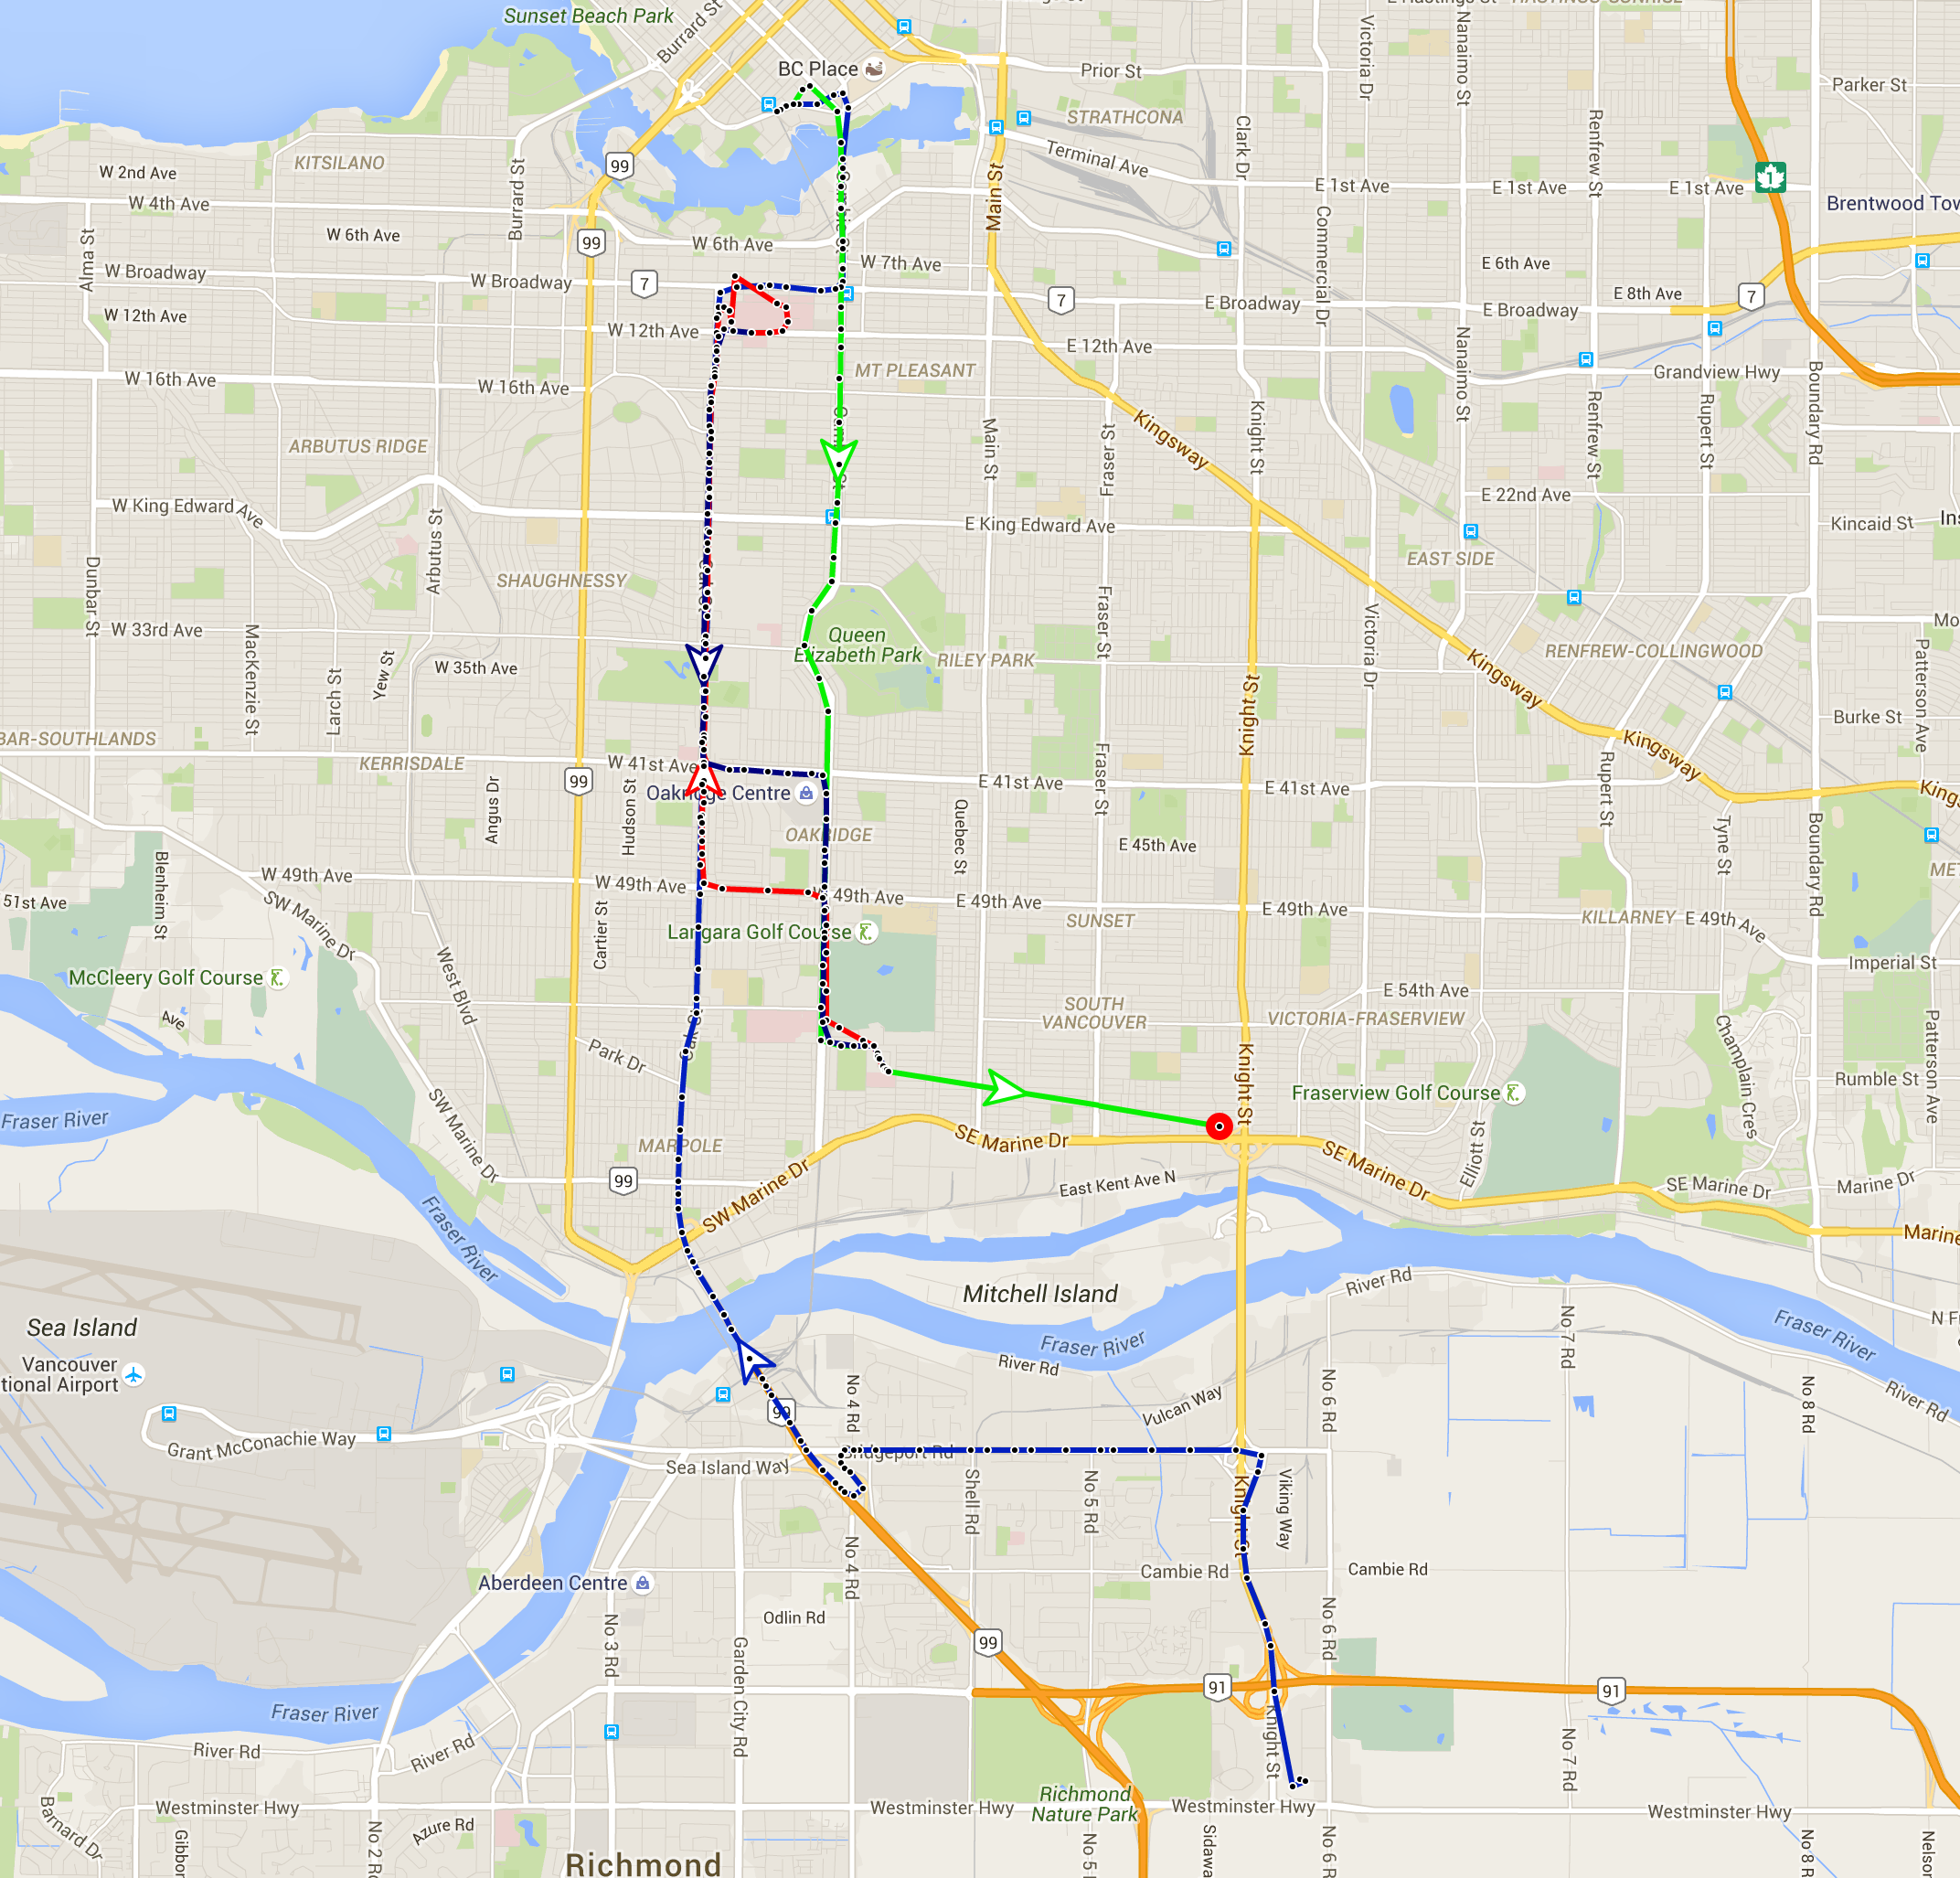
\includegraphics[width=0.7\textwidth]{figuras/Screen Shot 2016-05-12 at 3.25.21 PM.png}
    \caption{Mapa georreferenciado combinando dados de um GPS acoplado a um carro}
    \label{fig:mapa:georef}
\end{figure}
